% mnras_template.tex
%
% LaTeX template for creating an MNRAS paper
%
% v3.0 released 14 May 2015
% (version numbers match those of mnras.cls)
%
% Copyright (C) Royal Astronomical Society 2015
% Authors:
% Keith T. Smith (Royal Astronomical Society)

% Change log
%
% v3.0 May 2015
%    Renamed to match the new package name
%    Version number matches mnras.cls
%    A few minor tweaks to wording
% v1.0 September 2013
%    Beta testing only - never publicly released
%    First version: a simple (ish) template for creating an MNRAS paper

%%%%%%%%%%%%%%%%%%%%%%%%%%%%%%%%%%%%%%%%%%%%%%%%%%
% Basic setup. Most papers should leave these options alone.
\documentclass[a4paper,fleqn,usenatbib]{mnras}

% MNRAS is set in Times font. If you don't have this installed (most LaTeX
% installations will be fine) or prefer the old Computer Modern fonts, comment
% out the following line
\usepackage{newtxtext,newtxmath}
% Depending on your LaTeX fonts installation, you might get better results with one of these:
%\usepackage{mathptmx}
%\usepackage{txfonts}

% Use vector fonts, so it zooms properly in on-screen viewing software
% Don't change these lines unless you know what you are doing
\usepackage[T1]{fontenc}
\usepackage{ae,aecompl}

\usepackage{mhchem}



\usepackage{graphicx}
\usepackage{subcaption}
\usepackage{float}

\usepackage{color}
\usepackage{booktabs,chemformula}
\usepackage[export]{adjustbox}


\usepackage{tabularx}

\usepackage{caption}
\usepackage{subcaption}
\usepackage{amsmath}

\usepackage{tikz}
\usepackage{hyperref}

\usepackage{color}
\newcommand{\todo}[1]{\textcolor{red}{#1}}


\newcommand{\LamostGiants}{454180}
\newcommand{\project}[1]{\emph{#1}}
\newcommand{\lamost}{\project{LAMOST}

\newcommand{\teff}{T_{\rm eff}}
\newcommand{\logg}{\log_{10}[g\,({\rm cm\,s}^{-2})]}

%%%%%%%%%%%%%%%%%%% TITLE PAGE %%%%%%%%%%%%%%%%%%%

% Title of the paper, and the short title which is used in the headers.
% Keep the title short and informative.
\title[Short title, max. 45 characters]{Mg Depleted and K Enriched Stars from LAMOST Spectral Data}

% The list of authors, and the short list which is used in the headers.
% If you need two or more lines of authors, add an extra line using \newauthor
\author[Kemp et al.]{
Alex J. Kemp,$^{1}$\thanks{E-mail: ajkem1@student.monash.edu}
Andrew R. Casey,$^{1,2}$
%Matthew Miles? (Monash)
%Brodie Norfolk? (Monash)
%Amanda Karakas? (Monash)
%John Lattanzio? (Monash)
%Kevin Schlaufman? (JHU)
%Anna Ho? (Caltech)
\\
% List of institutions
$^{1}$School of Physics \& Astronomy, Monash University, Clayton 3800, Victoria, Australia\\
$^{2}$ Faculty of Information Technology, Monash University, Clayton 3800, Victoria, Australia\\
}

% These dates will be filled out by the publisher
\date{Accepted 2018 XX XX. Received 2018 YY YY; in original form 2018 ZZ ZZ}

% Enter the current year, for the copyright statements etc.
\pubyear{2018}


\begin{document}
\label{firstpage}
\pagerange{\pageref{firstpage}--\pageref{lastpage}}
\maketitle

% Abstract of the paper
\begin{abstract}
454180 RGB stars from the low resolution LAMOST DR2 survey were searched for anomalously high K and depleted Mg signatures. This study represents the largest search for field stars containing the Mg-K anti-correlation so far identified only in the globular NGC 2419 and NGC 2808. 23 stars displaying absorption spectra with over-abundant K and depleted Mg accross a range of metalicities were identified, but none were identified as having [Mg/Fe] or [K/Fe] consistent with the Mg depleted population found in NGC 2419. The abundances in these 23 stars are estimated at ranging between [INSERT RANGE FOR K AND MG HERE BASED OFF LAMOST DATA]. High resolution spectra for three stars (1 of which is not included among the final count of 23 spectral candidates for the signiature for reasons relating to the LAMOST signal quality for that star, despite having the highest K abundance of the three at [K/Fe]=1.54) selected based on observability characteristics were obtained using the Las Campanas Observatory, and for these stars elemental abundances for heavy elements such as Sc and V are also presented.
\end{abstract}

% Select between one and six entries from the list of approved keywords.
% Don't make up new ones.
\begin{keywords}
keyword1 -- keyword2 -- keyword3
\end{keywords}

%%%%%%%%%%%%%%%%%%%%%%%%%%%%%%%%%%%%%%%%%%%%%%%%%%

%%%%%%%%%%%%%%%%% BODY OF PAPER %%%%%%%%%%%%%%%%%%

\section{Introduction}

NGC 2419 is the Milky Way's third most massive globular cluster, and its chemical composition makes it perhaps the most unusual star cluster in the Galaxy. Recent spectroscopic studies of red giant branch (RGB) stars in NGC 2419 revealed a strong anti-correlation between Mg and K abundances in nearly half of the studied stars, and weaker abundance relations in Si, Sc, Ca, Ti and V \citep{mucciarelli2012,cohenkirby2012}. Depletions of Mg within globular clusters are not uncommon, but are always accompanied with an increase in [Fe/H] \todo{[citations needed; possibly remove]}. One mechanism for this phenomena is the introduction of $\alpha$-poor and Fe-rich material released from Type Ia supernovae which locally pollutes the more `normal' [Mg/Fe] ratios that arise from Type II supernovae. However, the two populations in NGC 2419 are indistinguishable in their [Fe/H] abundance \citep{cohenkirby2012}. Furthermore, Type Ia supernovae enrichment cannot account for the enhanced K abundance or the similar  abundance trends observed in NGC 2419.


Currently there is no known nuclear process that can explain the abundance variations in NGC 2419 without invoking unrealistic temperature conditions or by altering reaction rates by several orders of magnitude. 



%Recently \cite{youngwooklee} used a Ca filter to identify two population in NGC 2419 corresponding to two generations of stars: G1, first generation metal poor stars, and G2, second generation stars displaying enhanced Ca and significantly increased He abundance ($\Delta Y = 0.19$). The Mg depleted population identified previously was found to be contained with the G2 population.


The Mg-K anti correlation initially established in NGC 2419 continues to elude satisfactory explanation. Beyond the intrinsic scientific value of identifying the polluter object which is (presumably) responsible for the puzzling Mg-K anti-correlation, a satisfactory explanation for this signature could potentially offer insight into the underestimation of K abundance predicted by models \citep{kobayashi2011}. Such an explanation could also be beneficial to efforts to understand globular cluster formation and evolution.




It has been suggested that NGC 2419's position and size, being both very massive and very distant from the Milky Way compared to many other globular clusters, aids it in retaining enriched material from explosive events \citep{mucciarelli2012}. It is also perhaps noteworthy that NGC 2808 is also one of the more massive globular clusters of the Milky Way, although it is far closer to the Galactic Centre. But if this unknown pollution event is common among globular clusters and the cause of its apparent exclusivity to NGC 2808 and NGC 2419 is enhanced ejecta retention due to high mass, then other massive clusters such as $\omega$ Centauri would also be expected contain the signature, which to date has not been observed.


With the exception of NGC 2808, in which all 4 of its known Mg depleted stars have been found to have an anti-correlation with K \citep{mucciarelli2015}, this signature has thus far been found to be contained within NGC 2419. A  targeted search looking [K/Fe] in RGB stars from clusters NGC 6752, NGC 6121, NGC 1904, and $\omega$ Centauri as well as 21 field stars found in all cases K abundances falling within the bounds of the Mg normal population in NGC 2419 \citep{carretta2013}.



The fact that the Mg-K anti-correlation is confined to these very few specific globular clusters would seem to imply either a small population  of unusual polluter stars of some sort or a single extremely massive polluter star.

%While it is plausible that the increased mass and greater distance from the gaseous disk of the Milky Way would cause a clusters first generation polluter stars to have an increased effect on the second generation of stars, this effect would apply to all ejecta (assuming comparable energies). So while it might be expected that second generation stars in clusters similar to NGC 2419 made up of more material processed by the first generation than other lighter globular clusters, it doesn't explain why the ejecta from the first generation was apparently dominated by this as yet unknown polluter object resulting in the Mg-K anti-correlation. In the opinion of the author, it is the identity and physical characterisation of this unknown polluter that is of the greatest scientific interest, with such a result also hopefully answering the question of the signatures uniqueness.

%An early modelling attempt at replicating the anomalous abundances in NGC 2419 assumed hot-bottom burning in AGB and super-AGB (SAGB) stars \citep{ventura2012}. This study succeeded in reproducing the Mg-K anti-correlation, using the nuclear reaction pathway \ce{^{36}Ar(p,\gamma)^{37}K(\beta ^+ \nu)^{37}Ar(e^-,\nu)^{37}Cl(p,\gamma)^{38}Ar(p,\gamma)^39K} (corrected as per \cite{iliadis2016}) for nuclear synthesis of K. However, abundance patterns consistent with NGC 2419 were only attainable if the reaction cross section was set to 100 times the commonly accepted rate or temperatures could be made higher than currently accepted values, achieving a burning temperature of 150 MK. 

%A more recent, comprehensive attempt to replicate the Mg and K abundances in NGC 2419 by \cite{iliadis2016} also attempted to reproduce the abundances of Si, Sc, Ca, Ti and V (elements reported as having weak correlations with Mg by \cite{cohenkirby2012}). The ultimate goal was to constrain the temperatures and densities required to produce the chemical signiature, and thereby provide insight into potential polluter candidates. It is perhaps noteworthy that they identified a diferent main reaction pathway for K nucleosynthesis to that of \cite{ventura2012}, which is relegated to a minor minor seccondary pathway. The main pathway they identify is \ce{^{36}Ar(p,\gamma)^{37}K(\beta ^+ \nu)^{37}Ar(p,\gamma)^{38}K(\beta ^+ \nu)^{38}Ar(p,\gamma)^39K}. 

%It was found that (with the exception of extremely high densities > $10^8$ g/cm$^3$) temperatures between 100 and 200 MK and densities between 10$^{-4}$ and 10$^8$ g/cm$^3$ were required. Using this information, core and shell burning of low mass, high mass and super massive stars were ruled out as potential poluter candidates, as well as regular AGB stars. Super-AGB (SAGB) stars however were regarded as potential candidates, with only a relatively small (roughly 10-20 MK) increase in temperature required to fall in the acceptable band of parameter space identified. The other potential candidate identified was Novae, although the lack of detailed models of white dwarfs accreting material similar to NGC 2419 either from a binary companion or the intra cluster medium limit appraisals of its feasibility regarding whether enough ejecta could be produced and retained by the cluster. However, based on current novae frequency in globular clusters determined by \cite{kato2013novae}, \cite{iliadis2016} conclude that the amount of material that would be produced by Novae is at most 1 \% of the total required mass to pollute 30 \% of NGC 2419.

%Another proposed  polluter candidate is a pair instability super nova (PISN) \citep{carretta2013}. Unique to extremely massive population III stars, these events involve the total destruction of the star, with no black hole remnant being left behind. The main argument for this idea is that the extreme rarity of these events, coupled with the huge masses of processed material involved, could potentially allow the entire signature in NGC 2419 to be the result of a single event, explaining why it is not seen in any other globular clusters. Further, the signature odd-even proton number abundance pattern associated with PISNs could perhaps explain the anti-correlation between Mg and K, as well as the enhancements in Sc and V observed by \cite{cohenkirby2012}.

This study, which queries \LamostGiants\ \lamost\ giants for depleted Mg and enhanced K, seeks to provide additional information which can be used to guide and test models attempting to explain the Mg-K anti-correlation and related phenomena. The large sample size provides greater insight into the supposed exclusivity of the signature, and the stars identified present an important opportunity for follow up observations.


\section{Methods, Observations, Simulations etc.}

The data set of 454180 LAMOST giants was prepared by \citet{ho2017} for use with the supervised machine learning code \textit{The Cannon}. The LAMOST data was shifted to rest frame, normalised, and sampled to a common uniform wavelength grid between 3905 \AA \\ and 9000 \AA. \textit{The Cannon} was used to infer $\text{T}_{\text{eff}}$, log(g), [Fe/H] and [$\alpha$/M] using 9952 common stars between LAMOST and the higher resolution APOGEE survey through the use of a data-driven spectral model, referred to henceforth and simply 'the model'. For details regarding the preparatory work, model generation and label transfer between the APOGEE and LAMOST surveys, the reader is directed to \citet{ho2017}. The data-driven model generated by \textit{The Cannon} is treated in this study as the typical spectra for each star.

Residuals were taken of the normalised LAMOST flux data and 
\textit{The Cannon} according to $residual=data-model$. A positive residual therefore implies a higher normalised flux than expected by the model, while a negative residual implies a lower normalised flux than expected. In turn, at a given spectral line a lower normalised flux is associated with an over-abundance, while a higher normalised flux is associated with a depleted abundance.

A Gaussian curve was fitted to the residuals about each spectral line in the Mg triplet (5167 \AA, 5172 \AA, 5184 \AA) as well as the K doublet (7665 \AA, 7699 \AA) to characterise any deviation from the model. The amplitude and amplitude error for this curve was then used as the basis for a data filter designed to produce potential candidate stars with spectra indicative of Mg depletion, as well as K enrichment.

Three filters were applied independently, with the candidate pool formed from all unique stars identified each of the three filters. The first filter required the Mg 5184 line's Gaussian to satisfy $Amp > 0.05$ and $\frac{Amp}{Amp_{err}}>3$, and the K 7665 line to satisfy $Amp < 0.05$ and $\frac{Amp}{Amp_{err}}>3$. The second, more demanding filter was applied to require 2 of the three Mg lines to satisfy $Amp > 0.05$ and $\frac{Amp}{Amp_{err}}>3$, as well as either of the two K lines to satisfy $Amp < 0.05$ and $\frac{Amp}{Amp_{err}}>3$. The third filter removed the amplitude requirement to requiring only positivity on 2/3 Mg lines and negativity on \textit{both} K lines, in addition to data quality requirements $\chi^2<3$ and $S/N>30$.
These filters together produced 384 unique candidate stars to be vetted manually.

The vetting process was done through visual examination of each case. The minimum criterion for a pass was two out of the three Mg lines to look at least plausibly depleted, and at least one of the K lines to look convincing. The apparent noisiness of the signal was qualitatively taken into account when making these determinations. Of the 384 candidates manually vetted, 188 were ultimately determined to be sufficiently strong for further examination based on the spectra around the K and Mg lines.

The 6556 \AA \\ H line was then visually examined for each star to identify stars with active chromosphere emissions which could result in false positives for Mg depletion. 62 stars were removed from the sample due to being chromospheric emmiters. A further 13 stars were removed due to the model fitted poorly to the H 6556 line possibly due to incorrect log(g) or $\text{T}_{\text{eff}}$ estimates from \textit{The Cannon}, leaving a total of 113 candidates displaying depleted Mg and enhanced K.

\subsection{Figures and tables}

Figures and tables should be placed at logical positions in the text. Don't
worry about the exact layout, which will be handled by the publishers.

Figures are referred to as e.g. Fig.~\ref{fig:example_figure}, and tables as
e.g. Table~\ref{tab:example_table}.




\begin{figure}
	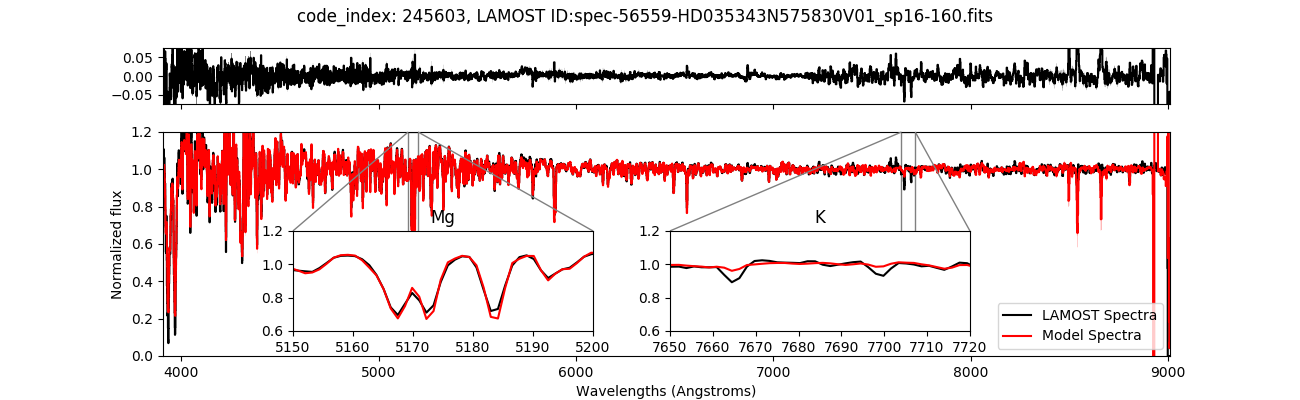
\includegraphics[width=\columnwidth]{posterchildof13.png}
    \caption{Poster Child}
    \label{mhist}
\end{figure}

\begin{figure}
	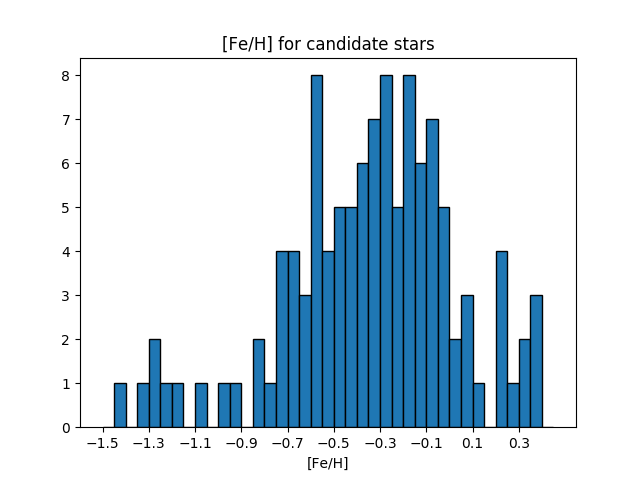
\includegraphics[width=\columnwidth]{histof113.png}
    \caption{Metalicity Histogram}
    \label{mhist}
\end{figure}


\begin{figure}
	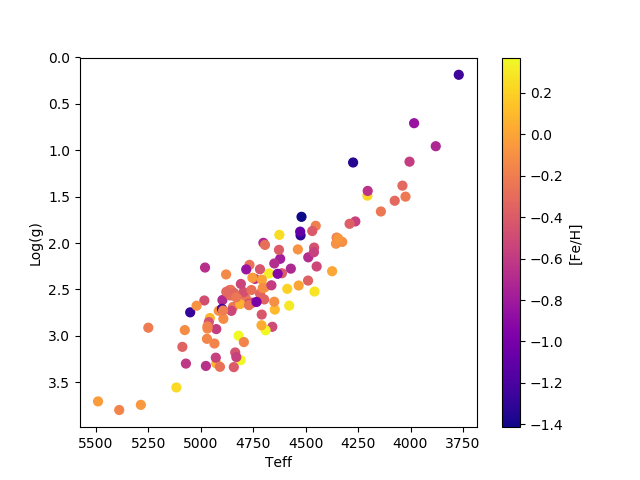
\includegraphics[width=\columnwidth]{loggteffof113.png}
    \caption{Effective temperature, log surface gravity, metalicity}
    \label{mhist}
\end{figure}

\begin{figure}
	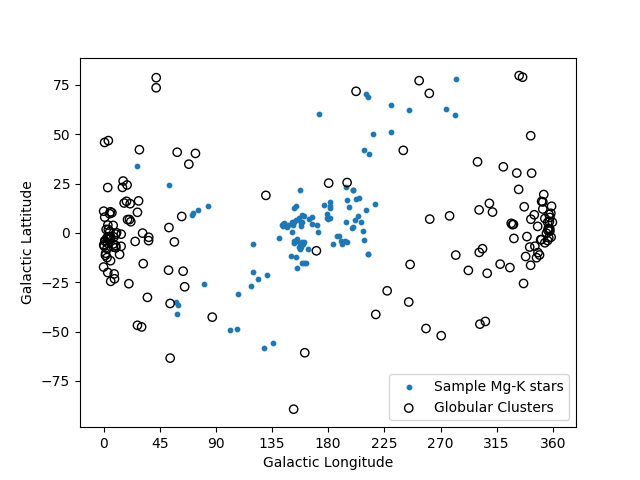
\includegraphics[width=\columnwidth]{globclustof113.png}
    \caption{Galactic coordinates for Mg-K stars and known globular clusters}
    \label{mhist}
\end{figure}

% Example table
\begin{table}
	\centering
	\caption{This is an example table. Captions appear above each table.
	Remember to define the quantities, symbols and units used.}
	\label{tab:example_table}
	\begin{tabular}{lccr} % four columns, alignment for each
		\hline
		A & B & C & D\\
		\hline
		1 & 2 & 3 & 4\\
		2 & 4 & 6 & 8\\
		3 & 5 & 7 & 9\\
		\hline
	\end{tabular}
\end{table}


\section{Conclusions}

The last numbered section should briefly summarise what has been done, and describe
the final conclusions which the authors draw from their work.

\section*{Acknowledgements}

The Acknowledgements section is not numbered. Here you can thank helpful
colleagues, acknowledge funding agencies, telescopes and facilities used etc.
Try to keep it short.

%%%%%%%%%%%%%%%%%%%%%%%%%%%%%%%%%%%%%%%%%%%%%%%%%%

%%%%%%%%%%%%%%%%%%%% REFERENCES %%%%%%%%%%%%%%%%%%

% The best way to enter references is to use BibTeX:

\bibliographystyle{mnras}
\bibliography{mgkbib} % if your bibtex file is called example.bib


% Alternatively you could enter them by hand, like this:
% This method is tedious and prone to error if you have lots of references


%%%%%%%%%%%%%%%%%%%%%%%%%%%%%%%%%%%%%%%%%%%%%%%%%%

%%%%%%%%%%%%%%%%% APPENDICES %%%%%%%%%%%%%%%%%%%%%

\appendix

\section{Some extra material}

If you want to present additional material which would interrupt the flow of the main paper,
it can be placed in an Appendix which appears after the list of references.

%%%%%%%%%%%%%%%%%%%%%%%%%%%%%%%%%%%%%%%%%%%%%%%%%%


% Don't change these lines
\bsp	% typesetting comment
\label{lastpage}
\end{document}

% End of mnras_template.tex